\documentclass[a4paper]{article}

\usepackage{enumitem}
\usepackage{mathtools}

\usepackage{bm}
\usepackage{url}

\usepackage{verbatim} 
\usepackage{enumitem}

\usepackage{relsize}
\usepackage{sectsty}

\usepackage{titlesec}
\titlespacing*{\section}{0pt}{0.2\baselineskip}{0.1\baselineskip}
\titlespacing*{\subsection}{0pt}{0.2\baselineskip}{0.1\baselineskip}
\titlespacing*{\subsubsection}{0pt}{0.2\baselineskip}{0.1\baselineskip}

\allsectionsfont{\smaller[1.5]}

\usepackage{tikz}
\usetikzlibrary{shapes,arrows}

\usepackage{amssymb}

\tikzstyle{block} = [draw, fill=blue!20, rectangle, 
    minimum height=3em, minimum width=6em]
\tikzstyle{sum} = [draw, fill=blue!20, circle, node distance=1cm]
\tikzstyle{input} = [coordinate]
\tikzstyle{output} = [coordinate]
\tikzstyle{pinstyle} = [pin edge={to-,thin,black}]

\usepackage{amsmath}
\usepackage{algorithm}
\usepackage[noend]{algpseudocode}

\makeatletter
\def\BState{\State\hskip-\ALG@thistlm}
\makeatother

\usepackage[
	per-mode=symbol,
	output-decimal-marker={,},
	separate-uncertainty=true,
]{siunitx}

\usepackage{booktabs}
\usepackage{caption}
\captionsetup[table]{skip=1ex}
\captionsetup[figure]{font=scriptsize}

\newenvironment{Figure}
  {\vspace{0pt}\noindent\minipage{\linewidth}}
  {\endminipage\vspace{5pt}}

% ------------------------------------------------

\usepackage[brazilian]{babel}
\usepackage[utf8]{inputenc}
\usepackage[none]{hyphenat}
\usepackage[T1]{fontenc}
\usepackage{amsfonts}
\usepackage{psfrag}
\usepackage{amssymb}
\usepackage{mathrsfs}
\usepackage{amsthm}
\usepackage{graphicx}
\usepackage{chngpage}
\usepackage{multicol}
\usepackage{multirow}
\usepackage{enumitem}
\usepackage[top=0.2in, bottom=0.2in, left=1cm, right=1cm]{geometry}
\setlength{\parskip}{0.2pt}

\linespread{1.1} %espaçamento 1.5
\newcommand{\bfg}[1]{\mbox{\boldmath $ #1 $}}
\newcommand{\mbf}[1]{\mathbf{#1}}
\newcommand{\bs}[1]{\boldsymbol{#1}}

\allowdisplaybreaks

%-----------------------------------------------------

\hyphenation{
to-po-lo-gi-a
To-po-lo-gi-a
re-so-lu-cao
di-fe-ren-tes
mi-ni-mi-zem
pro-ble-mas
mo-de-lo
ou-tros
pa-ra-le-lo
cons-tan-te
cons-tan-tes
me-lho-ra-ram
de-sen-vol-vi-men-to
cor-res-pon-den-te
as-so-ci-a-das
com-pa-ram
pla-ca
re-a-li-za
en-ge-nha-ri-a
}

\let\endtitlepage\relax

\title{

\vspace{-45pt}

\begin{figure}[htbp]
    \centering
        
\includegraphics[width=1\textwidth]{Imagem_PIBIC.png}
    \label{fig:logo}
\end{figure}
\vspace{-20pt}
  \textbf{\large{Estudo e Aplicação de Modelos de Previsão no Contexto de Séries de Vazões de Rios}}
\vspace{-5pt}
\begin{center}
  \normalsize{
  Aluno: Daniel da Costa Nunes Resende Neto 
  \\
  Orientador: Prof. Levy Boccato
  \\
  Faculdade de Engenharia Elétrica e de Computação (FEEC)
  }
\end{center}

\vspace{-45pt}

}

%Mantém em branco os campos Autor e Data
\date{}
\author{}

\begin{document}

\begin{titlepage}
 \maketitle
 \thispagestyle{empty}
\end{titlepage}


\sloppy
    
\begin{multicols}{2}
\raggedcolumns
\section{Introdução}
\label{sec:introducao}
    
    Uma série temporal é uma sequência de medidas feitas ao longo do tempo sobre um fenômeno de interesse. Em várias áreas do conhecimento, tais como engenharia, economia, matemática aplicada e computação, diversas séries temporais são particularmente relevantes não só pela perspectiva de análise e interpretação de seus históricos passados, mas também pela possibilidade de estimar seus valores futuros. Este último desafio dá origem ao problema de predição de séries temporais \cite{Box-Jenkins}.
    
    Um cenário em que este problema aparece com destacada importância está associado a séries de vazões de rios. Neste contexto, a disponibilidade de previsões confiáveis a respeito do volume disponível de água pode ser decisiva para um planejamento energético mais eficiente e seguro para uma determinada região. Isso se torna ainda mais relevante quando a principal fonte de geração de energia é hídrica, a partir das usinas hidrelétricas, como é o caso do Brasil.
    
    Neste trabalho, foram estudados dois modelos lineares de predição clássicos da literatura: auto-regressivo (AR) e auto-regressivo de médias móveis (ARMA) \cite{Box-Jenkins}. No caso do modelo ARMA, exploramos uma meta-heurística denominada \textit{clearing} \cite{Levy2010, goldberg} para o ajuste de seus parâmetros, visando minimizar o erro quadrático médio na etapa de treinamento.
    
    Foram considerados também métodos não-lineares baseados em redes neurais artificiais \cite{Geron}. São eles: a rede \textit{perceptron} de múltiplas camadas (MLP, do inglês \emph{multilayer perceptron}), como representante da classe de modelos \emph{feedforward}, assim como três modelos recorrentes: as RNNs (do inglês, \emph{recurrent neural networks}) simples, as LSTMs (do inglês, \emph{long short-term memory}) \cite{LSTM} e as GRUs (do inglês, \emph{gated recurrent units}) \cite{GRU2}.
    
    Todos os modelos foram aplicados às séries de vazões de Água Vermelha e Jirau (ver Seção \ref{subsec:serie}), e, por fim, comparados a partir do Erro Quadrático Médio (EQM) gerado para os dados de teste de ambas as séries. A metodologia completa, os resultados obtidos e as conclusões finais do projeto encontram-se nas Seções \ref{subsec:comparacao_modelos} e \ref{sec:conclusoes} deste documento.

\section{Modelos de Previsão}
\label{sec:modelos_nao_lineares}

\subsection{Modelos Lineares}

\subsubsection{AR} \label{subsubsec:AR_descricao}

O modelo mais clássico de previsão é o auto-regressivo (AR, do inglês \emph{auto-regressive}) \cite{Box-Jenkins,Haykin}.
    No AR , o valor da série no instante $n$, aqui denotado por $x(n)$, é determinado a partir de uma combinação linear dos valores passados até um instante $n-M-L+1$, onde $M$ determina a ordem do modelo e $L$ o passo de previsão (quantos instantes de tempo à frente pretende-se estimar). Em termos matemáticos, a regra de evolução temporal do modelo AR é dada por:
    \begin{equation}
        x(n) = a_1 x(n-L) + \ldots + a_M x(n-M-L+1) + \eta(n)
    \label{eq:ar}
    \end{equation}
    onde $a_i, i = 1,\ldots,M$ são os coeficientes do modelo AR que ponderam as amostras passadas da série e $\eta(n)$ denota o erro instantâneo, cuja média é nula e cuja variância ($\sigma_{\eta}^2$) é constante. Este último termo constitui um ruído branco (em inglês, \emph{white noise}) \cite{Box-Jenkins}.
    
\subsubsection{ARMA} \label{subsubsec:ARMA_descricao}
    
    O modelo ARMA (do inglês, \emph{auto-regressive moving-average}) \cite{Box-Jenkins, Haykin} gera a estimativa do valor da série no instante $n$ a partir de uma combinação linear de valores passados da própria série, como ocorre no AR, e de amostras passadas do ruído branco (ou, analogamente, do erro de predição), como mostra a expressão abaixo:
    \begin{equation}
        x(n) = \sum_{k=0}^{M} a_k x(n-k-L+1) + \sum_{k=0}^{K} b_k\eta(n-k-J+1)
    \label{eq:arma}
    \end{equation}
    onde $b_0 = 1$, $J$ e $K$ são o passo e o número de atrasos do ruído branco, respectivamente, e as definições dadas para o modelo AR ainda valem.
    
    Passaremos, agora, à apresentação dos fundamentos teóricos dos modelos não-lineares utilizados no trabalho.
    
\subsection{Modelos Não-lineares}

    A definição de uma rede neural artificial passa pelas escolhas: (1) do modelo de neurônio, bem como (2) de sua função de ativação, (3) da arquitetura da rede, tipicamente organizada em camadas, e (4) dos valores mais apropriados para os hiperparâmetros, como o número de camadas e a quantidade de neurônios em cada camada. A seguir, apresentamos brevemente as estruturas estudadas neste trabalho. 
    
\subsubsection{MLP}
\label{subsubsec:mlp_descricao}
    
    As MLPs são redes neurais formadas fundamentalmente por múltiplas camadas de neurônios artificiais \cite{Geron}, os quais recebem os atributos $x_i$ contidos na instância $\mathbf{x}$ e os ponderam pelos pesos $w_i \subset \mathbf{w}$ do neurônio. Aplica-se, então, uma função de ativação $\phi$ sobre esta soma ponderada, acrescida de um termo de \textit{bias} (\textit{b}), de forma a gerar a saída:
\begin{equation}
\begin{aligned}
h_{\mathbf{w}}(\mathbf{x}) = \phi\left(\sum_{i=1}^{n}w_ix_i + b\right)
\end{aligned}
\label{eq:saida_na}
\end{equation} 

    A função de ativação $\phi$ pode assumir várias formas, sendo as mais utilizadas as funções: logística, tangente hiperbólica (Tanh), ReLu e SeLu \cite{Geron}.

    Uma MLP é composta, primeiramente, por uma camada ($l = 0$) de entrada. Os neurônios desta camada apenas passam para suas saídas o  atributo com o qual foram alimentados. As próximas camadas, exceto a última, são denominadas camadas intermediárias (em inglês, \emph{hidden layers}). Em cada camada, os estímulos de entrada são combinados linearmente, com base nos pesos de cada neurônio, e a função de ativação é aplicada sobre o resultado acumulado, conforme a Equação \eqref{eq:saida_na}. Assim, cada uma das saídas dos neurônios de uma camada é propagada adiante para cada um dos neurônios da próxima camada, até que cheguem à última camada da rede. 
    
    Por fim, a camada de saída (em inglês, \emph{output layer}) é quem gera as respostas da rede para uma instância. No treinamento da rede, discutido mais a diante, as instâncias são apresentadas à rede agrupadas em um \textit{mini-batch}.
    
    A Equação \eqref{eq:saida_na} pode ser generalizada matricialmente (ver expressões em \eqref{eq:MLP}) para definir a matriz contendo os vetores de saídas de uma camada gerados a partir de uma sequência de vetores de entrada. Isto é feito separadamente para a camada de entrada (equação \eqref{eq:entrada}), uma camada intermediária (equação \eqref{eq:saida_intermediaria}) e a camada de saída (equação \eqref{eq:saida_ultima}). Essa representação possibilita o cálculo da matriz de saída de uma rede alimentada com um subconjunto de instâncias chamado \textit{mini-batch}. Ela é utilizada no treinamento da rede (abordado em breve).
\begin{subequations}
\begin{align}
& \mathbf{H}^0(\mathbf{X}) = \mathbf{X}, \label{eq:entrada}\\
& \mathbf{H}_{\mathbf{W^l,B^l}}^l(\mathbf{H}^{l-1}) = \phi(\mathbf{H}^{l-1}\mathbf{W}^l + \mathbf{B}^l), \label{eq:saida_intermediaria}\\
& \mathbf{H}_{\mathbf{W^L,B^L}}^L(\mathbf{H}^{L-1}) = \phi(\mathbf{H}^{L-1}\mathbf{W}^L + \mathbf{B}^L) \label{eq:saida_ultima}
\end{align}
\label{eq:MLP}
\end{subequations}
Nestas equações: 
\begin{itemize}[noitemsep]
    \item A matriz $\mathbf{X} = [\mathbf{x}_1 \,\, \mathbf{x}_2 \,\, \dots \,\, \mathbf{x}_d]^\top$, com $\mathbf{X} \in \mathbb{R}^{d \times n}$, é o \textit{mini-batch} recebido pela rede e contém $d$ instâncias $\mathbf{x}_i^\top$ em suas linhas, sendo que cada instância é caracterizada por $n$ atributos; 
    \item Os vetores coluna $\mathbf{w}_j^l$ da matriz $\mathbf{W}^l = [\mathbf{w}_1^l \,\, \mathbf{w}_2^l \,\, \dots \,\, \mathbf{w}_{m(l)}^l]$, com $\mathbf{W}^l \in \mathbb{R}^{m(l-1) \times m(l)}$, contêm os conjuntos de pesos pertencentes a cada um dos $m(l)$ neurônios da camada $l$. Note que o número de pesos de um neurônio da camada $l$ (a dimensão dos vetores $\mathbf{w}_j^l$) é igual ao número de neurônios da camada anterior $m(l-1)$, já que este é também seu número de saídas. Os valores assumidos por $m(l)$ quando $l = 1, ..., L$ são definidos na construção da rede e, como as saídas da camada de entrada são as próprias entradas, $m(0) = n$; 
    \item A matriz $\mathbf{H}^l = [\mathbf{y}_{1}^l \,\, \mathbf{y}_{2}^l \,\, \dots \,\, \mathbf{y}_{d}^l]^\top$, com $\mathbf{H}^l \in \mathbb{R}^{d \times m(l)}$, contém os $d$ vetores linha de saídas $\mathbf{y}_{i}^{l \top}$ da camada $l$. Cada um deles contém $m(l)$ saídas;
    \item Cada vetor $\mathbf{b}_{i}^{l}$ na matriz $\mathbf{B}^l = [\mathbf{b}_{1}^l \,\, \mathbf{b}_{2}^l \,\, \dots \,\, \mathbf{b}_{d}^l]^\top$, com $\mathbf{B}^l \in \mathbb{R}^{d \times m(l)}$, especifica o \textit{bias} de cada neurônio da camada $l$, contendo $d$ cópias deste valor;
    \item A função de ativação $\phi$ é aplicada a todos os elementos da matriz $(\mathbf{H}^{l-1}\mathbf{W}^l + \mathbf{B}^l)_{d \times m(l)}$, gerando, assim, as respostas dos neurônios da camada $l$. 
\end{itemize}

\subsubsection{RNN}
\label{subsubsec:RNNsimples_descricao}

Uma RNN apresenta uma estrutura bastante similar à de uma MLP, mas com a presença de retroalimentações. Deste modo, a cada instante de tempo $t$ (também chamado de \emph{frame}), esta rede recebe o vetor de entradas $\mathbf{x}_{(t)}$ juntamente com o próprio vetor de saídas do instante de tempo anterior, $\mathbf{y}_{(t-1)}$.

    Sendo assim, cada neurônio recorrente possui dois vetores de pesos: o primeiro, $\mathbf{w}_x$, pondera as entradas instantâneas $\mathbf{x}_{(t)}$; o segundo, $\mathbf{w}_y$, é responsável por ponderar as saídas passadas, $\mathbf{y}_{(t-1)}$. Considerando agora uma camada recorrente, podemos agrupar todos os pesos em duas matrizes, $\mathbf{W}_x$ e $\mathbf{W}_y$, de maneira que o vetor de saída da camada pode ser escrito como:
\begin{equation}
\begin{aligned}
\mathbf{y}_{(t)} = \phi\,(\mathbf{x}_{(t)}^\top\mathbf{W}_x + \mathbf{y}_{(t-1)}^\top\mathbf{W}_y + \mathbf{b}^\top)^\top
\label{eq:RNN_camada_padrão}
\end{aligned}
\end{equation}
sendo $\mathbf{b}$ o vetor de \textit{bias}. 

De modo análogo ao que foi feito para a MLP, podemos agrupar várias instâncias em um único \textit{mini-batch} $\mathbf{X}_{(t)}$, de modo que a matriz de saídas é dada por: 
\begin{equation}
\begin{aligned}
\mathbf{Y}_{(t)} &= \phi\,(\mathbf{X}_{(t)}\mathbf{W}_x + \mathbf{Y}_{(t-1)}\mathbf{W}_y + \mathbf{B}) \\
&= \phi\,(\left[\begin{array}{cc}
\mathbf{X}_{(t)} & \mathbf{Y}_{(t-1)}\\
\end{array}\right]\mathbf{W}  + \mathbf{B}) \, \text{,} \, \, \mathbf{W} = \left[\begin{array}{c}
\mathbf{W}_{x} \\
\mathbf{W}_{y}\\
\end{array}\right]
\label{eq:RNN_camada_batch}
\end{aligned}
\end{equation}
onde a matriz $\mathbf{Y}_{(t)}$ contém em cada linha as saídas de uma instância do \textit{mini-batch}; a matriz $\mathbf{X}_{(t)}$ contém em cada linha uma instância de tamanho igual à quantidade de atributos; as matrizes $\mathbf{W}_{x}$ e $\mathbf{W}_{y}$ contêm em cada coluna os pesos que multiplicam os atributos e as saídas prévias de uma instância, respectivamente; a matriz $\mathbf{B}$ contém o mesmo vetor de \textit{bias} de cada neurônio em cada uma de suas linhas; e as matrizes $\mathbf{W}_{x}$ e $\mathbf{W}_{y}$ podem ser concatenadas em uma única matriz $\mathbf{W}$, como mostrado.

Devido à relação de recorrência presente em \eqref{eq:RNN_camada_batch}, $\mathbf{Y}_{(t)}$ é, em tese, influenciado por todas as entradas desde $t = 0$, \textit{i.e.}, $\mathbf{X}_{(0)}, \mathbf{X}_{(1)},\ldots, \mathbf{X}_{(t)}$. Por isso, diz-se que a rede recorrente possui memória. A parte da rede que preserva estados ao longo do tempo é chamada de célula de memória (ou simplesmente célula).

A estrutura aqui apresentada (uma RNN simples) é uma célula muito básica, capaz apenas de aprender padrões curtos. As LSTMs e GRUs, apresentadas nas seções seguintes, buscam justamente a expansão desta memória temporal.

\subsubsection{LSTM}
\label{subsubsec:lstm_descricao}

Vista de fora, uma célula LSTM pode ser utilizada analogamente a um neurônio recorrente simples. A diferença é que seu estado é dividido em dois vetores diferentes: o vetor de longo prazo $\mathbf{c}$ e o vetor de curto-prazo $\mathbf{h}$. A estrutura interna de uma célula LSTM está representada na Figura \ref{fig:LSTM}.

\begin{Figure}
\centering
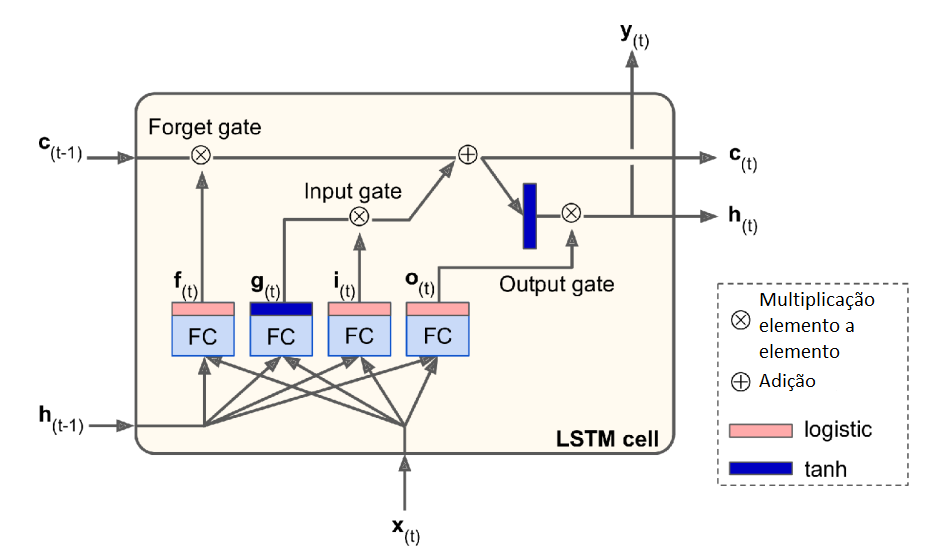
\includegraphics[width=\linewidth]{LSTM.png}
\captionof{figure}{Estrutura interna de uma célula LSTM. Figura adaptada de \cite{Geron}.}
\label{fig:LSTM}
\end{Figure}

Já as equações em \eqref{eq:LSTM} mostram como computar a saída da célula, bem como seus estados, no instante $t$ para um \textit{mini-batch}:
\begin{subequations}
\begin{align}
&\mathbf{I}_{(t)} = \sigma(\mathbf{X}_{(t)}\mathbf{W}_{xi} + \mathbf{H}_{(t-1)}\mathbf{W}_{hi} + \mathbf{B}_i) \\
&\mathbf{F}_{(t)} = \sigma(\mathbf{X}_{(t)}\mathbf{W}_{xf} + \mathbf{H}_{(t-1)}\mathbf{W}_{hf} + \mathbf{B}_f) \\
&\mathbf{O}_{(t)} = \sigma(\mathbf{X}_{(t)}\mathbf{W}_{xo} + \mathbf{H}_{(t-1)}\mathbf{W}_{ho} + \mathbf{B}_o) \\
&\mathbf{G}_{(t)} = \text{tanh}(\mathbf{X}_{(t)}\mathbf{W}_{xg} + \mathbf{H}_{(t-1)}\mathbf{W}_{hg} + \mathbf{B}_g) \\
&\mathbf{C}_{(t)} = \mathbf{F}_{(t)} \otimes \mathbf{C}_{(t-1)}^{\top} + \mathbf{I}_{(t)} \otimes \mathbf{G}_{(t)}^{\top} \\
&\mathbf{Y}_{(t)} = \mathbf{H}_{(t)} = \mathbf{O}_{(t)} \otimes \text{tanh} (\mathbf{C}_{(t)}^{\top})
\end{align}
\label{eq:LSTM}
\end{subequations}
A primeira alteração que ocorre no estado de longo prazo do instante anterior $\mathbf{c}_{(t-1)}$ é a perda de parte de sua memória na chamada porta de esquecimento (do inglês, \emph{forget gate}). Em seguida, é feita a incorporação de novas memórias pela porta de entrada (do inglês, \emph{input gate}), formando o vetor $\mathbf{c}_{(t)}$ (equação (7e)).
Uma cópia deste estado é filtrada pela porta de saída (do inglês, \emph{output gate}) e gera o estado de curto prazo $\mathbf{h}_{(t)}$ (equação (7f)), que também representa a saída da célula naquele instante. 

Agora, olharemos para a entrada da LSTM. O vetor $\mathbf{g}_{(t)}$ é a saída da camada principal (equação (7d)). As partes mais relevantes de  $\mathbf{g}_{(t)}$ são guardadas no vetor $\mathbf{c}_{(t-1)}$, e as menos relevantes descartadas.

Deste modo, o vetor $\mathbf{f}_{(t)}$ consegue controlar quais partes do vetor $\mathbf{c}_{(t-1)}$ devem ser apagadas (equação (7b)). O vetor $\mathbf{i}_{(t)}$ consegue controlar quais partes de $\mathbf{g}_{(t)}$
devem ser adicionadas ao vetor $\mathbf{c}_{(t-1)}$ (equação (7a)). Finalmente, o vetor $\mathbf{o}_{(t)}$ seleciona quais partes de $\mathbf{c}_{(t-1)}$ devem formar tanto a saída $\mathbf{y}_{(t)}$ quanto o estado de curto-prazo $\mathbf{h}_{(t)}$ (equação (7c)).

Resumidamente, uma célula LSTM é capaz de detectar uma entrada relevante (pela porta de entrada), guardá-la no vetor de estado a longo prazo o quanto for necessário (pela porta do esquecimento) e extraí-la quando necessário (pela porta de saída). Isso traz à tona a capacidade elevada (em relação a uma célula recorrente simples) de reconhecimento e preservação de tendências presentes, no contexto deste projeto, em série temporais.

\subsubsection{GRU}
\label{subsubsec:gru_descricao}

A célula GRU é uma versão simplificada da célula LSTM, e funciona de modo análogo. Sua estrutura interna está representada na Figura \ref{fig:GRU}.

\begin{Figure}
 \centering
 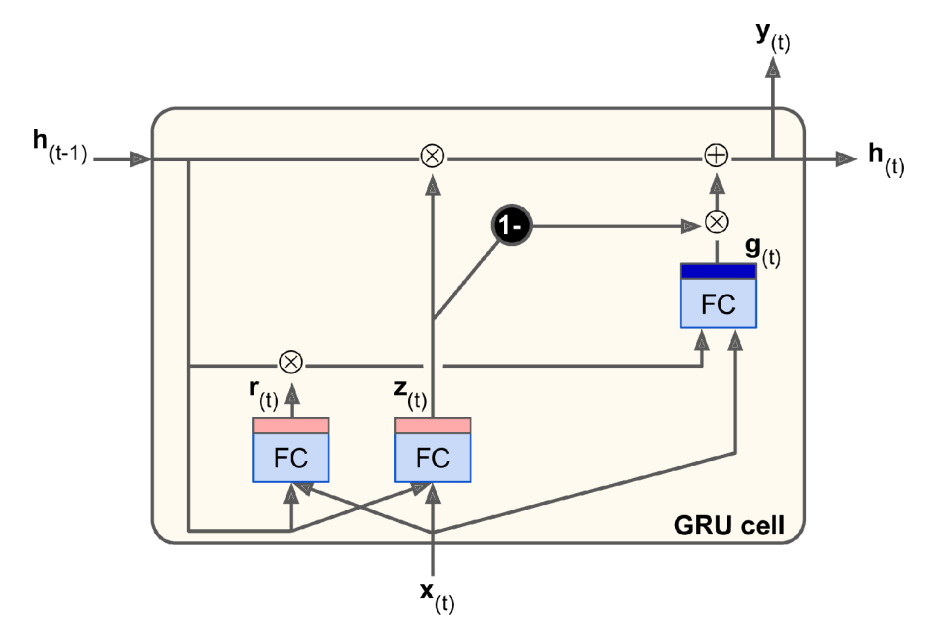
\includegraphics[width=\linewidth]{GRU.png}
\captionof{figure}{Estrutura interna de uma célula GRU. Figura adaptada de \cite{Geron}.}
\label{fig:GRU}
\end{Figure}

Como pode ser observado, há agora somente um vetor de estado, $\mathbf{h}$. Além disso, um único vetor $\mathbf{z}_{(t)}$ controla tanto a porta de esquecimento (\textit{forget gate}) quanto a porta de entrada (\textit{input gate}). Em outras palavras, para que uma memória seja mantida, o conteúdo do local em questão deve ser primeiramente apagado.

Além disso, não existe mais uma porta de saída (\textit{output gate}). Contudo, existe agora o vetor $\mathbf{r}_{(t)}$, o qual decide qual parte do vetor de estado prévio $\mathbf{h}_{(t-1)}$ será mostrado à camada principal (de saída $\mathbf{g}_{(t)}$). É importante notar que a capacidade de memória de uma LSTM ou de uma GRU ainda é limitada, de modo que o aprendizado de padrões bastante afastados no tempo pode ser difícil.

\subsubsection{Treinamento}

Para que uma rede seja treinada, é necessário encontrar os valores de todos os pesos sinápticos, $\mathbf{W}^l, l = 1, \ldots, L$, que minimizem uma medida de erro (neste caso, o EQM) entre as saídas geradas pela rede e as saídas desejadas. 

No caso da MLP, utiliza-se o algoritmo de retropropagação do erro (em inglês, \textit{error backpropagation}) para o cálculo das derivadas da função custo com respeitos aos parâmetros de toda a estrutura \cite{Haykin}. Já para a RNN, aplica-se a retropropagação do erro através do tempo (do inglês, \emph{backpropagation through time}).

O otimizador clássico utilizado na atualização dos pesos da rede é o gradiente descendente \cite{Geron}. Contudo, a otimização por gradiente descendente pode sofrer com o desaparecimento dos gradientes (em inglês, \textit{vanishing gradients problem}), ou ainda o contrário: o seu aumento desenfreado (em inglês, \textit{exploding gradients problem}), que é mais comum no contexto de redes recorrentes.

Uma técnica desenvolvida para tentar evitar ambos os problemas supracitados é a normalização do  \textit{batch} (BN, do inglês \emph{batch normalization}) \cite{Geron}. Ela consiste na adição de uma operação dentro do modelo logo antes ou depois da aplicação da função de ativação em cada camada intermediária.

Esta operação simplesmente centraliza todas as instâncias ao redor do zero e as normaliza. Para isso, o algoritmo deve estimar a média e o desvio padrão de cada atributo dentro do \textit{mini-batch} (daí o nome) que alimenta a camada de BN. Isso é feito da seguinte maneira:
\begin{subequations}
\begin{align}
&\bm{\mu}_B = \frac{1}{d} \sum^{d}_{i=1} \mathbf{x}_i \label{eq:bn_1}\\
&\bm{\sigma}_B^2 = \frac{1}{d} \sum^{d}_{i=1} (\mathbf{x}_i - \bm{\mu}_B )^2 \label{eq:bn_2}\\
&\mathbf{\hat{x}}_i = \frac{\mathbf{x}_i - \bm{\mu}_B }{\sqrt{\bm{\sigma}_B^2 + \epsilon}} \label{eq:bn_3}\\ 
&\mathbf{z}_i = \bm{\gamma} \otimes \mathbf{\hat{x}}_i + \bm{\beta} \label{eq:bn_4}
\end{align}
\end{subequations}
onde $\bm{\mu}_B$ e $\bm{\sigma}_B$ são os vetores contendo, respectivamente, a média e o desvio padrão de cada atributo para o \textit{mini-batch}; $\mathbf{\hat{x}}_i$ é a \textit{i}-ésima instância centrada em zero e normalizada; $\bm{\gamma}$ é o vetor que pondera cada um dos atributos normalizados em $\mathbf{\hat{x}}_i$; $\otimes$ representa o produto elemento a elemento; o vetor $\bm{\beta}$ contém o \textit{offset} relativo a cada atributo normalizado; $\epsilon$ é um número pequeno que impede a divisão por zero (tipicamente $10^{-5}$); e $\mathbf{z}_i$ é a saída reescalada e deslocada da camada de \textit{batch normalization}.

O uso de BN introduz dois novos parâmetros por camada: um que escala os atributos normalizados $\bm{\gamma}$ e outro que os desloca $\bm{\beta}$. Cabe ao modelo aprender a escala e o deslocamento ótimo de cada atributo para cada camada.

Outro problema característico do gradiente descendente é sua lentidão, a qual pode ser contornada com a utilização de outros otimizadores. O otimizador explorado neste trabalho é o Nadam (do inglês, \emph{Nesterov adaptive moment estimation}). O conjunto de equações que o descreve é dado por:
\begin{subequations}
\begin{align}
&\mathbf{w}' = \mathbf{w} + \beta_3\mathbf{m} \label{eq:nadam_0} \\
&\mathbf{m} \gets \beta_1\mathbf{m} - (1-\beta_1) \nabla_{\mathbf{w}}E(\mathbf{w}') \label{eq:nadam_1}\\
&\mathbf{s} \gets \beta_2\mathbf{s} - (1-\beta_2) \nabla_{\mathbf{w}}E(\mathbf{w}') \otimes \nabla_{\mathbf{w}}E(\mathbf{w}') \label{eq:nadam_2}\\
&\mathbf{\hat{m}} \gets \frac{\mathbf{m}}{1 - \beta_1} \label{eq:nadam_3}\\ 
&\mathbf{\hat{s}} \gets \frac{\mathbf{s}}{1 - \beta_2} \label{eq:nadam_4} \\
&\mathbf{w} \gets \mathbf{w} + \eta \mathbf{\hat{m}} \oslash \sqrt{\mathbf{\hat{s}} + \epsilon} \label{eq:nadam_5}
\end{align}
\end{subequations}

A otimização por momento presente no Nadam incorpora a influência de gradientes passados, não apenas o local. Isto é feito subtraindo-se o gradiente local, desta vez, do vetor de momento $\mathbf{m}$ (ver equação \eqref{eq:nadam_1}). E este, por sua vez, é utilizado para atualizar o peso $\mathbf{w}$ (veja a equação \eqref{eq:nadam_5}). 

O gradiente passa, então, a transmitir a ideia de aceleração, e não mais velocidade. Assim, o algoritmo acumula velocidade de convergência caso esteja caminhando para um ótimo local e escapa de platôs mais rapidamente.

Para que o algoritmo não avance velozmente em uma direção que não aponta para o ótimo local (como acontece no metódo clássico do gradiente descendente), introduz-se o vetor $\mathbf{s}$ (ver equação \eqref{eq:nadam_2}), o qual escala o vetor momento (ver equação \eqref{eq:nadam_5}). 

Por fim, o Nadam também incorpora a ideia proposta pelo matemático Yurii Nesterov (daí o nome) de que o gradiente deve ser medido não sobre o ponto atual $\mathbf{w}$, mas sobre um ponto levemente à frente na direção do vetor momento, como faz a equação \eqref{eq:nadam_0}. Esta ideia pode ser benéfica, uma vez que o vetor de momento geralmente aponta na direção correta (a direção do ponto ótimo), tornando a atualização dos pesos mais precisa.

Nas próximas seções, apresentaremos características relevantes da séries de vazões, bem como a metodologia de treinamento aplicada. Concomitantemente, os resultados obtidos com os modelos lineares e não-lineares na etapa de teste serão relatados, analisados e, ao final, comparados entre si.

\section{Metodologia e Resultados}
\label{sec:metodologia}
    
\subsection{Descrição das Séries e Divisão de Dados}
\label{subsec:serie}
    
    As séries de vazões fluviais diárias (em $m^3/s$) utilizadas neste projeto foram as das usinas de Água Vermelha e Jirau, considerando-se um período de 16 anos: de $1^\text{o}$ de janeiro de 2000 a 31 de dezembro de 2015.
    
    Os primeiros 5114 dias ($1^\text{o}$ de janeiro de 2000 a 31 de dezembro de 2013) constituíram os dados de treinamento e validação, os quais foram fornecidos aos modelos de previsão. Já os últimos 730 dias ($1^\text{o}$ de janeiro de 2014 a 31 de dezembro de 2015) foram usados na etapa de teste.
    
    Os perfis hidrológicos destas séries são significativamente diferentes, trazendo variedade à análise dos métodos de previsão empregados.

\subsection{Implementação}
\label{subsec:implementacao}

    A mesma metodologia foi aplicada durante o projeto e avaliação dos modelos, de modo a tornar a comparação de seus respectivos desempenhos verossímil. A implementação dos modelos foi dividida em duas etapas: validação e teste.
    
\begin{enumerate}[noitemsep]
  \item \textbf{Etapa de Validação}
  \begin{enumerate}[label*=\arabic*.]
    \item Escolhem-se números $M$ de atrasos (valores passados da respectiva série) pertencentes a um intervalo $I_M$ (definido a partir da função de autocorrelação parcial das séries), e treinam-se os modelos com validação cruzada (do inglês, \textit{cross validation}) do tipo \textit{holdout} ou $k$-\textit{fold}. Para as redes neurais, especificamente, varia-se concomitantemente o número $N$ de neurônios na camada intermediária. Ademais, também foram testadas diferentes funções de ativação, inicializações, taxas de aprendizado e a presença (ou ausência) de BN. Já para o modelo ARMA, são considerados, também, números $K$ de atrasos (valores passados dos erros cometidos) pertencentes a um intervalo $I_K$ (definido a partir da função de autocorrelação das séries).
  \end{enumerate}
  \item \textbf{Etapa de Teste}
  \begin{enumerate}[label*=\arabic*.]
    \item Ao final do treinamento, as melhores configurações de cada modelo são retreinadas, com ou sem validação, e utilizadas para prever múltiplas vezes todas as vazões presentes nos dados de teste (de $1^\text{o}$ de janeiro de 2014 a 31 de dezembro de 2015) da série em questão. A média dos EQMs cometidos para os dados de teste é a medida do desempenho daquele modelo na previsão da respectiva série.
  \end{enumerate}
\end{enumerate}
    
\subsection{Comparação entre modelos} 
\label{subsec:comparacao_modelos}

As melhores combinações de parâmetros de cada modelo e seus respectivos EQMs para os dados de teste são colocados na Tabela \ref{tab:resultados_finais} em ordem crescente.

\begin{table*}[t]
\centering
\caption{Configuração ótima e desempenho de teste dos modelos de previsão para as séries de Água Vermelha e Jirau.}
\label{tab:resultados_finais}
\begin{tabular}{lcccccccc}
\toprule
Modelo & M & K & N & Água Vermelha $(m^3/s)^2$ & M & K & N & Jirau $(m^3/s)^2$ \\
\midrule
RNN simples & 5 & - & 20 & $1048 \pm 110$ & 4 & - & 5 & $414914 \pm 11516$\\
ARMA & 5 & 1 & - & $1056,\!3$ & 5 & 1 & - & $614060$ \\
GRU & 10 & - & 100 & $1088 \pm 98$ & 9 & - & 100 & $502325 \pm 40190$ \\
AR & 29 & - & - & $1088,\!6$ & 2 & - & - & $393130$ \\
MLP & 8 & - & 10 & $1165 \pm 79$ & 4 & - & 5 & $478170 \pm 6554$ \\
LSTM & 8 & - & 150 & $1322 \pm 100$ & 22 & - & 100 & $456127 \pm 20792$ \\
\bottomrule
\end{tabular}
\vspace{-6mm}
\end{table*} 

O primeiro ponto a ser destacado é que o desempenho das células recorrentes foi superior ao desempenho da MLP. Consideremos uma MLP com uma única camada de $N_n$ neurônios. Esta rede contém, para instâncias de tamanho $n$, $n \times N_n$  pesos a serem ajustados. Já uma rede recorrente de camada única, e mesmo número de neurônios, necessita apenas ajustar $N_n$ parâmetros (independentemente do tamanho da instância), pois estes são compartilhados entre os $n$ instantes de tempo. O número reduzido de pesos da rede recorrente simplifica um pouco seu aprendizado.

Quanto ao acesso das redes à instância, de fato, a MLP a observa por completo, enquanto a rede recorrente acessa somente um de seus elementos em cada instante de tempo. A informação introduzida por cada um desses elementos é passada para os instantes de tempo subsequentes somente por meio do estado da célula, dificultando a assimilação de padrões longos. Contudo, como as instâncias apresentam um tamanho $n \in I_M$ reduzido, a célula de memória consegue aprender com êxito os padrões fundamentais presentes na instância. Isto minimiza a suposta vantagem possuída pela MLP, de acesso à instância completa, e configura outro motivo pelo qual o desempenho da RNN simples foi superior.

Por outro lado, tanto a LSTM quanto a GRU não ofereceram melhorias em relação à RNN simples. Apesar de serem capazes de manter uma informação dentro da rede por um período de tempo mais longo, provavelmente nos cenários aqui tratados tal memória de longo prazo não era estritamente necessária. Assim, houve um gasto de recursos com uma arquitetura mais flexível que provou ser infrutífero para a otimização destas células. Deste modo, ambas as propostas (LSTM e GRU) acabaram sendo superadas pela RNN simples. 

Os modelos lineares, por sua vez, se saíram muito bem. O estudo feito em \cite{makridakis} mostra que modelos estatísticos (como o AR e o ARMA) podem superar métodos de aprendizado de máquina (ML, em inglês \emph{machine learning}), cuja sofisticação e demanda computacional são maiores. Isso mostra que um alto desempenho de extrapolação é acompanhado de grande eficiência. Em outras palavras, uma capacidade superior de predição pode ser atingida a partir de uma menor complexidade computacional. O inverso também é verdadeiro, já que abordagens mais complexas de extrapolação por métodos de ML exibem resultados piores, indicando que robustez teórica nem sempre é favorável.

O estudo \cite{makridakis} também mostra que modelos que melhor ajustam os parâmetros da rede durante o treinamento não necessariamente apresentam maior capacidade de extrapolação. O exemplo dado pelo artigo é a LSTM, a qual ``comparada com redes neurais mais simples, como a RNN e a MLP, demonstrou melhor \emph{fitting}, porém pior precisão de predição [para os dados de teste]''. Comparando-se, neste projeto, o desempenho de validação da LSTM ao desempenho de validação da RNN simples, nota-se esse mesmo comportamento: os EQMs de validação da LSTM são, no geral, menores, porém a capacidade de extrapolação da RNN simples é superior no contexto de ambas as séries.

Em suma, as características das séries de Água Vermelha e Jirau foram bem representadas pelos modelos lineares AR e ARMA, uma vez que este obteve o segundo menor EQM ($1056,\!3 \,\, (m^3/s)^2$) no contexto da série de Água Vermelha, e aquele obteve o menor EQM ($393130 \,\,(m^3/s)^2$) no contexto da série de Jirau. Já a flexibilidade adicional dos modelos não-lineares acabou dificultando o aprendizado efetivo dos comportamentos das séries, com exceção da RNN simples, a qual apresentou um desempenho equiparável ao dos modelos lineares: o menor EQM final ($1048 \pm 110 \,\, (m^3/s)^2$) no contexto da série de Água Vermelha e o segundo menor EQM final ($414914 \pm 11516 \,\, (m^3/s)^2$) no contexto da série de Jirau.
    
\section{Conclusões}
\label{sec:conclusoes}

    Neste trabalho, modelos estatísticos lineares e algumas estruturas não-lineares de redes neurais foram estudados e aplicados à predição de séries de vazões de rios, seguindo as práticas usuais em aprendizado de máquina para a correta validação e teste. 
    
\begin{Figure}
 \centering
 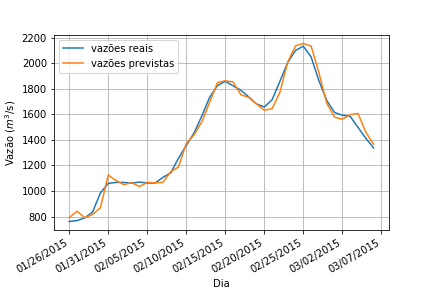
\includegraphics[width=\linewidth]{saidas_vazoes_zoom_RNN.png}
\captionof{figure}{Vazões previstas e vazões reais de Água Vermelha - RNN simples}
\label{fig:previsao_RNN}
\end{Figure} 
    
    Os modelos lineares e a RNN simples se destacaram como os mais adequados na resolução do problema de extrapolação, uma vez que a RNN simples apresentou o menor EQM final no contexto da série de Água Vermelha, e o AR apresentou o menor EQM final no contexto da série de Jirau.

    A título de ilustração, apresentamos as Figuras \ref{fig:previsao_RNN} e \ref{fig:previsao_AR} com as respectivas estimativas da RNN simples e do AR, durante o período de 1 (um) mês, para os dados de teste das séries de Água Vermelha e Jirau, respectivamente.
    
\begin{Figure}
 \centering
 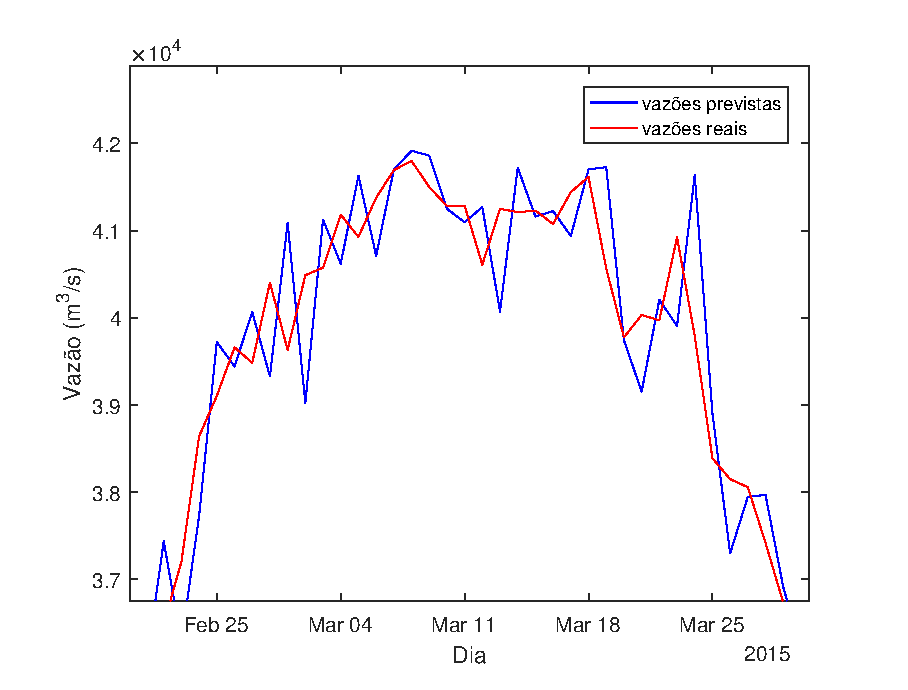
\includegraphics[width=\linewidth]{vazoes_Jirau_AR_zoom.eps}
\captionof{figure}{Vazões previstas e vazões reais de Jirau - AR}
\label{fig:previsao_AR}
\end{Figure}

    Deste modo, concluímos com êxito a proposta de trabalho, a qual colocou o aluno em contato com variadas técnicas modernas de ML.

%---------------------------------------------------------------------------
\bibliographystyle{myIEEEtran}
\small{
\bibliography{referencias_IC}}


%\bibitem{Box-Jenkins} Box, G.E.P. and Jenkins, G.M. "Time-Series Analysis: Forecasting and Control", Holden-Day, San Francisco, 1970.

%\vspace{2.0in}
%
%\newcommand{\HS}[1][1.]{\hspace{\stretch{#1}}}
%\begin{center}
%\ \hrulefill\ \HS[.2] \hrulefill\ \\
%\HS[.03]\  Levy Boccato - Candidato\ \HS[.3] Romis Attux - Supervisor\
%\end{center}


%---------------------------------------------------------------------------
\end{multicols}

\end{document}

